\documentclass[11pt]{article}
\usepackage[utf8]{inputenc}
\usepackage[english]{babel}
\usepackage[margin=1in]{geometry} 
\usepackage{graphicx}
\usepackage{xcolor}
\usepackage{sectsty}
\usepackage{hyperref}

\title{Human-Computer Interaction - Project Report\\A.A. 2018/2019}

\author{Matteo Franzil}

\hypersetup{%
  colorlinks=false,% hyperlinks will be coloured
  linkcolor=black,% hyperlink text will be green
  linkbordercolor=black,% hyperlink border will be red
}

\makeatletter
\Hy@AtBeginDocument{%
  \def\@pdfborder{0 0 1}% Overrides border definition set with colorlinks=true
  \def\@pdfborderstyle{/S/U/W 1}% Overrides border style set with colorlinks=true
                                % Hyperlink border style will be underline of width 1pt
}
\makeatother

\begin{document}

\maketitle

\section{Executive summary}

Sustainable mobility refers to the use of either non-polluting travel methods (e.g., walking or cycling), collective travel methods (e.g., bus, train, or car-pooling) or low-pollution travel means (e.g., electrical cars).

The goal of this project is to design a mid-fidelity prototype of a system that would encourage people to increase their use of sustainable mobility options.

This project is wholly focused on the Trentino region, especially in the city of Trento, where all interviewees study or work. This allowed me to ask more thorough questions, and to be more specific during the prototype creation.

I chose to create an all-around application, easily accessible by all users, that would promote multi-modal transport and last-mile transit options. This application would be able to replace most ones on the market, which have overlapping features but lack in key areas (such as real-time arrivals) or are poorly mantained.

This approach would encourage brand loyalty for both new and existing users, especially if the app were to be appropriately promoted. During the interviews, I realised that a great share of people wasn't fully aware of sustainable transport opportunities in Trento, so I thought that it would be advisable to cater to this "undecided" part of the population, rather than accustomed car-users which would never swap their veichle out.

The first prototype was hand-drawn on a tablet, printed and interactively shown to a group of people. They thoroughly tested the prototype, nit-picked as much as possible and highlighted critical areas. I used their feedback to improve the prototype, finally creating a medium-fidelity one on Adobe XD, which is the one presented at the end of this report.

\section{Analysis of existing solutions}
To start off, I looked at current options offered to citizens for encouraging the use of sustainable means of transport. In the autonomous province of Trento, most systems are specialized in \textit{alternative} means of transport, different than both buses and trains.

For example, around the city of Trento, bike sharing stations are available, both from \textbf{e.motion} and \textbf{C'entro in bici}. The former provides both regular and electric bikes with yearly and multi-day subscriptions, the latter supplies the user with a key which unlocks any bike, but forces the user to return it in the same spot within the day.

Regarding the usage of buses and coaches, \textbf{Trentino trasporti} is the local transport provider, handling buses, coaches, cableways and trains. For customers, applications such as \textbf{OpenMove} are available, offering purchase and usage of travel solutions within the app, while others are still in development (an application, made by the Province, is undergoing beta testing and will offer real-time information for buses and coaches using GPS localization), and others seem under-utilized or in need of revamping (such as \textbf{Viaggia Trento}). I noticed that while the wide variety of options is encouraging, it increases fragmentation and leads to user confusion.

To further promote the usage of public transport, game-like initiatives (rewarding users for their usage of sustainable means of transport, usually in a competitive way with leaderboards) showed up over the years, a notable presence being \textbf{Viaggia Play and Go}; however, their usage seems limited to a restricted age group, mainly the youth, since as the age increases so does the unwillingness to change one's daily habits or engaging in this type of activities.

Finally, Trentino also offers options to people who still prefer to use a car. Car sharing is becoming prevalent, with services provided by \textbf{Car Sharing Trentino}. Moreover, for people in possession of an electric car, recharge stations are starting to pop up, provided by \textbf{Dolomiti Energia} and \textbf{Trentino trasporti}.

I concluded that while various options are present, and most people using a car are hard to completely convert to public transport in a short time frame, what is missing in the picture is something similar to \textbf{Moovit} or \textbf{Citymapper}: an all-around application, powered by the Province, with a clear, consistent and accessible interface, to present users with \textit{all} options available for moving around, from bike and car sharing stations to bus stops with real time arrivals, and a search engine able to match these options up.

\section{Idea generation}

I decided to implement this idea focusing on one keyword, \textbf{simplicity}. The user interface has to be the same across platforms, with information clearly available avoiding sub-menus or visual clutter, in order to enable anyone to use the application regardless of their age.

The application will therefore focus into:
\begin{itemize}
    \item providing users with information on their surroudings, such as bus stops, bike and car sharing stations;
    \item enabling users to validate their ticket or unlock their rented bike;
    \item providing alternative ways of transport when searching for directions, such as complementing a train trip with a last-mile option such as a shared bike.
\end{itemize}

While most of these options are already available in existing apps, the goal is to remove accessibility and usability barriers and to promote usage of shared transport as a last-mile option, in areas poorly served by public transport and where walking is unfeasible or too slow. By maximing the amount of users, so will the amount of people aware of alternative means of transport in their territory.

\section{Interview results and diagrams}

I interviewed a wide variety of people, mainly inquiring about their attitude, use and views on public transport (including infrastructure, agencies, delays and services), their proficiency with a smartphone, and their usage of last-mile options.

In general, especially older people, commuters (may them be students or workers) tend not to rely on timetables or mobile applications at all, since they already know their trip by heart. Younger people and infrequent public transport users, on the other hand, are more likely to be heavy users of public transport apps, mainly \textit{OpenMove} (for university students), \textit{Google Maps}, or any other reliable or fast app for the purpose.

Most people, however, tended to agree that information about public transport is often somewhat limited or badly promoted, at least in the Trento area. A major percentage of the interviewees never picked up a shared bike or car, and a fraction of them didn't even know how to rent one. While bus stops are often well-equipped with timetables, the QR codes (linking to a website offering transport information) printed on them are almost always disregarded.

In the following pages flow (Figure \ref{fig:flow}), cultural (Figure \ref{fig:cultural}), artifact (Figure \ref{fig:artifact}), physical (Figure \ref{fig:physical}) and sequence (Figure \ref{fig:sequence}) diagrams are shown.

\begin{figure}[h!]
    \centering
    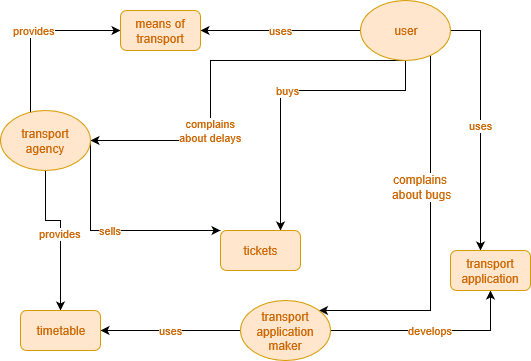
\includegraphics[width=0.8\textwidth]{drawable/diagrams/flow}
    \caption{Flow diagram}
    \label{fig:flow}
\end{figure}

\begin{figure}[h!]
    \centering
    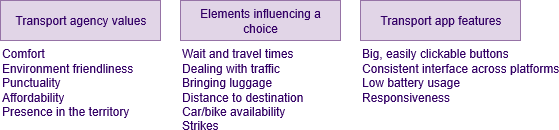
\includegraphics[width=0.8\textwidth]{drawable/diagrams/culture}
    \caption{Cultural diagram}
    \label{fig:cultural}
\end{figure}

\begin{figure}[h!]
    \centering
    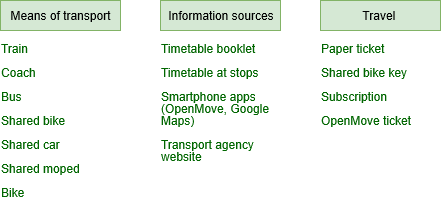
\includegraphics[width=0.7\textwidth]{drawable/diagrams/artifact}
    \caption{Artifact diagram}
    \label{fig:artifact}
\end{figure}

\begin{figure}[h!]
    \centering
    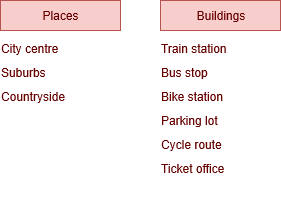
\includegraphics[width=0.5\textwidth]{drawable/diagrams/physical}
    \caption{Physical diagram}
    \label{fig:physical}
\end{figure}

\begin{figure}[h!]
    \centering
    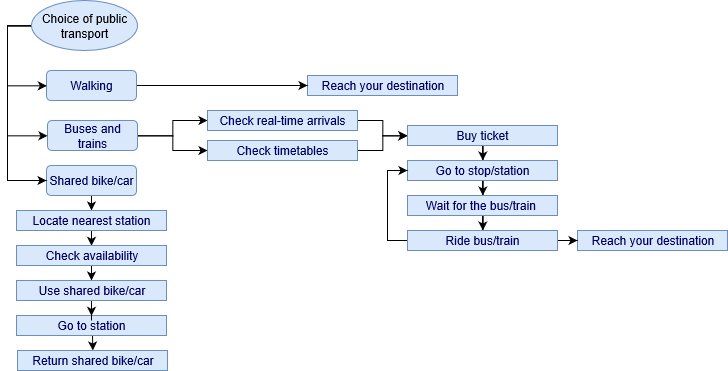
\includegraphics[width=0.8\textwidth]{drawable/diagrams/sequence}
    \caption{Sequence diagram}
    \label{fig:sequence}
\end{figure}

\newpage\newpage
\section{Personas}
In the following section, four different personas that I identified during the interview process are shown.
\par
%\begin{multicols}{2}
\textbf{Giacomo} - 21, university student
\begin{itemize}
    \item has a bus subscription and rides the bus daily to university
    \item is quite proficient with his smartphone
    \item uses OpenMove for validating his ticket, but knows timetables by heart
    \item if buses are late, happily walks or accepts a car lift
\end{itemize}
\par
\textbf{Teresa} - 58, worker
\begin{itemize}
    \item lives in the city centre and walks everyday to work, sometimes uses her bike
    \item knows the bare basics of her smartphone
    \item prefers checking paper timetables at the bus stop
    \item has heard of bike and car sharing but never thought about trying
\end{itemize}
\par
%\end{multicols}%\begin{multicols}{2}
\textbf{Thomas} - 39, worker
\begin{itemize}
    \item has to travel between cities frequently for work
    \item uses his smartphone a lot, also always carrying a PC with him
    \item has various travel apps to aid him while traveling
    \item sometimes resorts to car sharing while traveling in bigger cities
\end{itemize}
\par
\textbf{Gemma} - 80, old lady
\begin{itemize}
    \item seldom goes out, usually for grocery shopping
    \item does not own a smartphone and does not plan to buy one
    \item uses paper booklets to consult timetables before taking the bus
    \item used to own a driving licence and does not plan to use a bike anymore
\end{itemize}
%\end{multicols}

\section{Market gap}

At the end of the interviews, I concluded that while the market is flooded with both first and third party options for public transit, the lion's share of the interviewees either did not make use of one, or found out that most options had overlapping features but failed at delivering all of them: one application for the timetables, one for shared bikes, one for trains.

I also noticed that the general public has poor to zero usage of shared bikes: most interviewees agreed that it is a system with a tough entry barrier and additional costs that most people are not happy to accept.

In order to both raise awareness for these low-usage last mile options and to further build confidence on major transit options such as buses and trains, the general public needs an app that can \textit{replace} all of them.

\section{User requirements}

\subsection{Functional requirements}
\begin{itemize}
    \item Calculate directions to any point within the local area, including all transport options such as walking and last-mile options.
    \item Map view of the surroudings with bus stops, train stations and facilities, along with timetables and real-time arrivals.
    \item Purchase and validation of tickets and subscriptions.
\end{itemize}

\subsection{Non-functional requirements}

\begin{itemize}
    \item Clear, consistent interface with big, visible buttons - as suggested by Sofia, 22 years old, student.
    \item Easy to use for all age groups.
    \item As fast and reactive as possible, maybe working from the web too - as suggested by Tommaso, 25 years old, worker.
    \item Fast and high priority ticket validation, as fast as opening the smartphone camera.
    \item Transit directions that change depending on traffic and delays, just like Google Maps
\end{itemize}

\begin{figure}[h!]
    \centering
    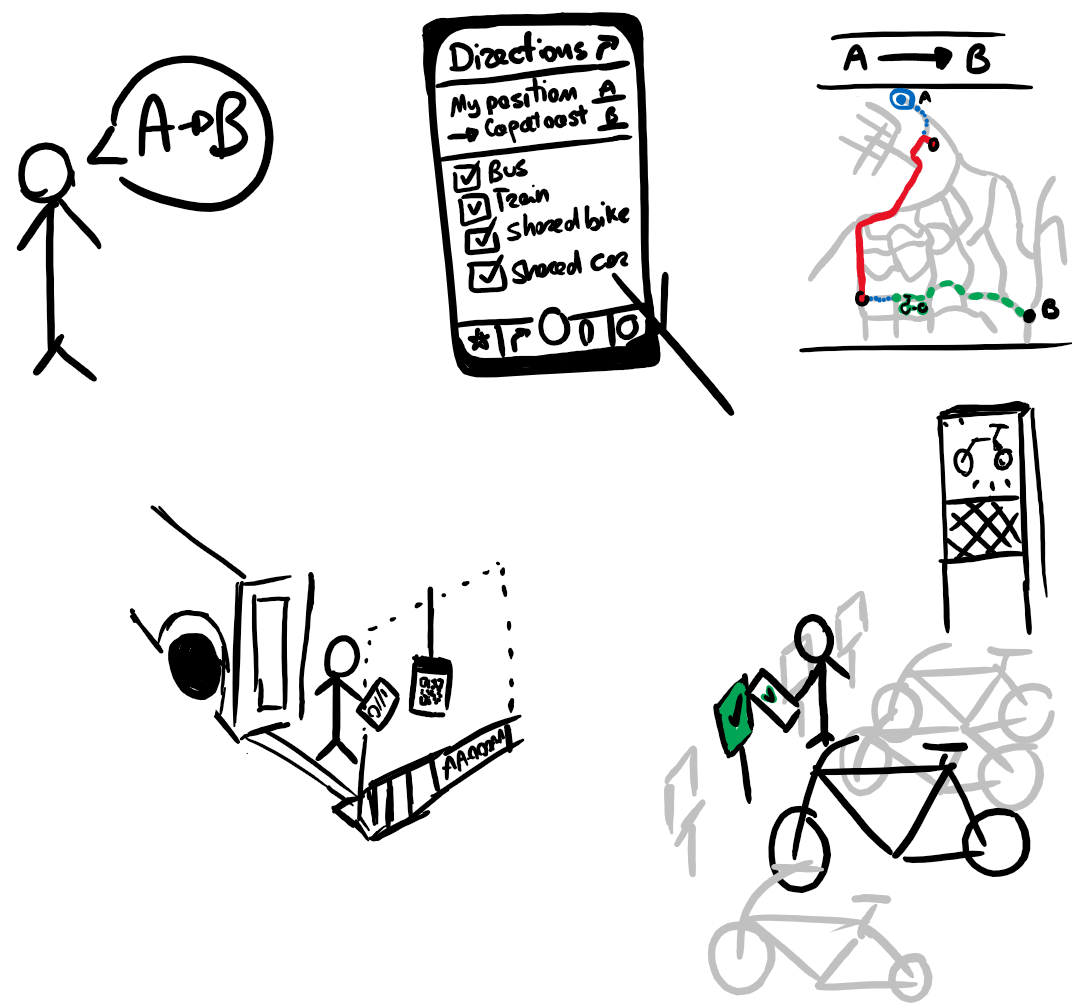
\includegraphics[width=0.5\textwidth]{drawable/usecase/usecase2}
    \caption{Use case for getting directions from A to B.}
    \label{fig:usecase}
\end{figure}

The design will be the main focus of the application. I want the application to appeal to as much people as possible, thus it will be important to use a big font, big buttons, and a bottom-navigation system in order to use it with only one hand.

The application will also need to implement a "favorites" system for easy access to one's frequently used bus stops and stations.

In the use case scenario shown in Figure \ref{fig:usecase}, the user who needs to move from point A to point B, first of all opens the application, locates the Directions tab, inserts his destination and receives a multi-modal trip including a bus ride and a shared bike last-mile journey. In the first case he validates his ticket with a QR code, in the second case he unlocks a bike using the phone's NFC capabilities (if present).

\section{Low fidelity prototype}

\begin{figure}[p]
    \centering
    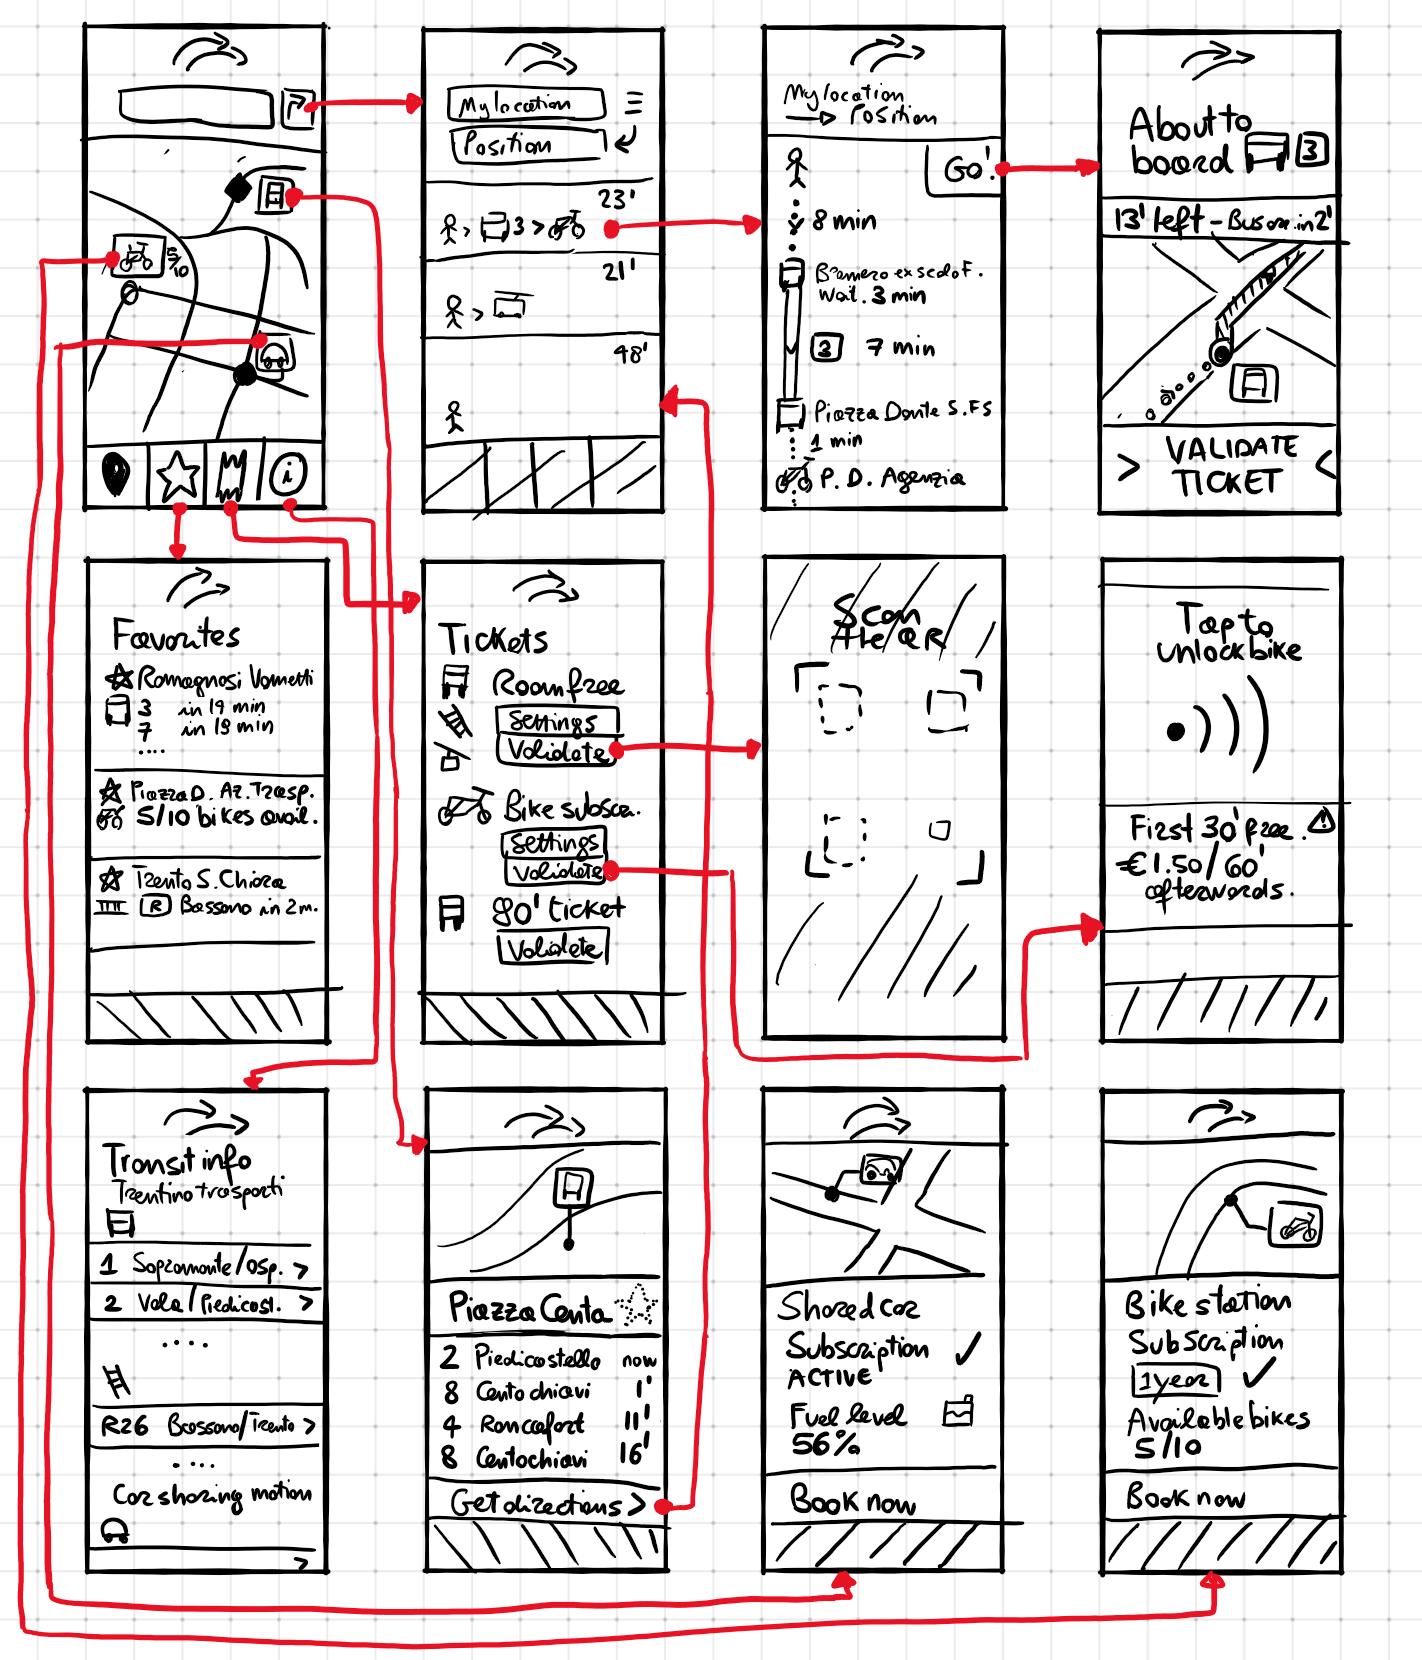
\includegraphics[width=\textwidth]{drawable/lowfid/lowfid2}
    \caption{Low fidelity prototype.}
    \label{fig:lowfid}
\end{figure}

Figure \ref{fig:lowfid} shows the low-fidelity prototype. A higher quality version can be found \href{https://drive.google.com/file/d/1eWlhHMJbUJPAnKBKt9aLeZLrWKuwrQIy/view?usp=sharing}{by clicking here,} or at this url:\\\url{https://drive.google.com/file/d/1eWlhHMJbUJPAnKBKt9aLeZLrWKuwrQIy/view?usp=sharing}

A trip within the application can be started in two ways, by manually inputting the destination or by clicking on the map (via the bus stop view, for example). In either way the application will suggest you some trip solutions. After having chosen one, the application tracks you during the whole trip, and suggests you to validate your ticket once reached the bike station or the bus has arrived.

Additional menus are available for manual ticket validation, information checking, favorites selection, and settings. All of them are accessible with one hand, using the navigation menu persent in the lower part of the screen. In general, most features are accessible with one or two taps without confusing sub-menus.

\section{Evaluation of the low fidelity protoype}

I tested the prototype against 5 people: I printed the prototype on paper and let the testers interact with it, changing views when necessary.

People praised the app's UI and found it intuitive for the most part. However, some parts of the apps were deemed cluttered, such as the Tickets view (some users said they didn't understand the tickets were already bought) and the Favorites view.

After analysing the testers' feedback, I came up with the following changes:

\begin{itemize}
    \item Ticket validation would be more practical with a button positioned in the navigation menu, without having to go through the Tickets menu. Therefore, a new button will be placed in every view for quick validation, while the Tickets view will feature an option for buying tickets;
    \item NFC bike unlocking would need a QR code counterpart to truly support all smartphones, as some models do not support it;
    \item The Directions view is confusing, and needs more focus on the remaining time and trip;
    \item The Favorites view is too cluttered, and could be converted to a list of stations which expands on click.
\end{itemize}

\section{Medium fidelity prototype}

\begin{figure}[p]
    \centering
    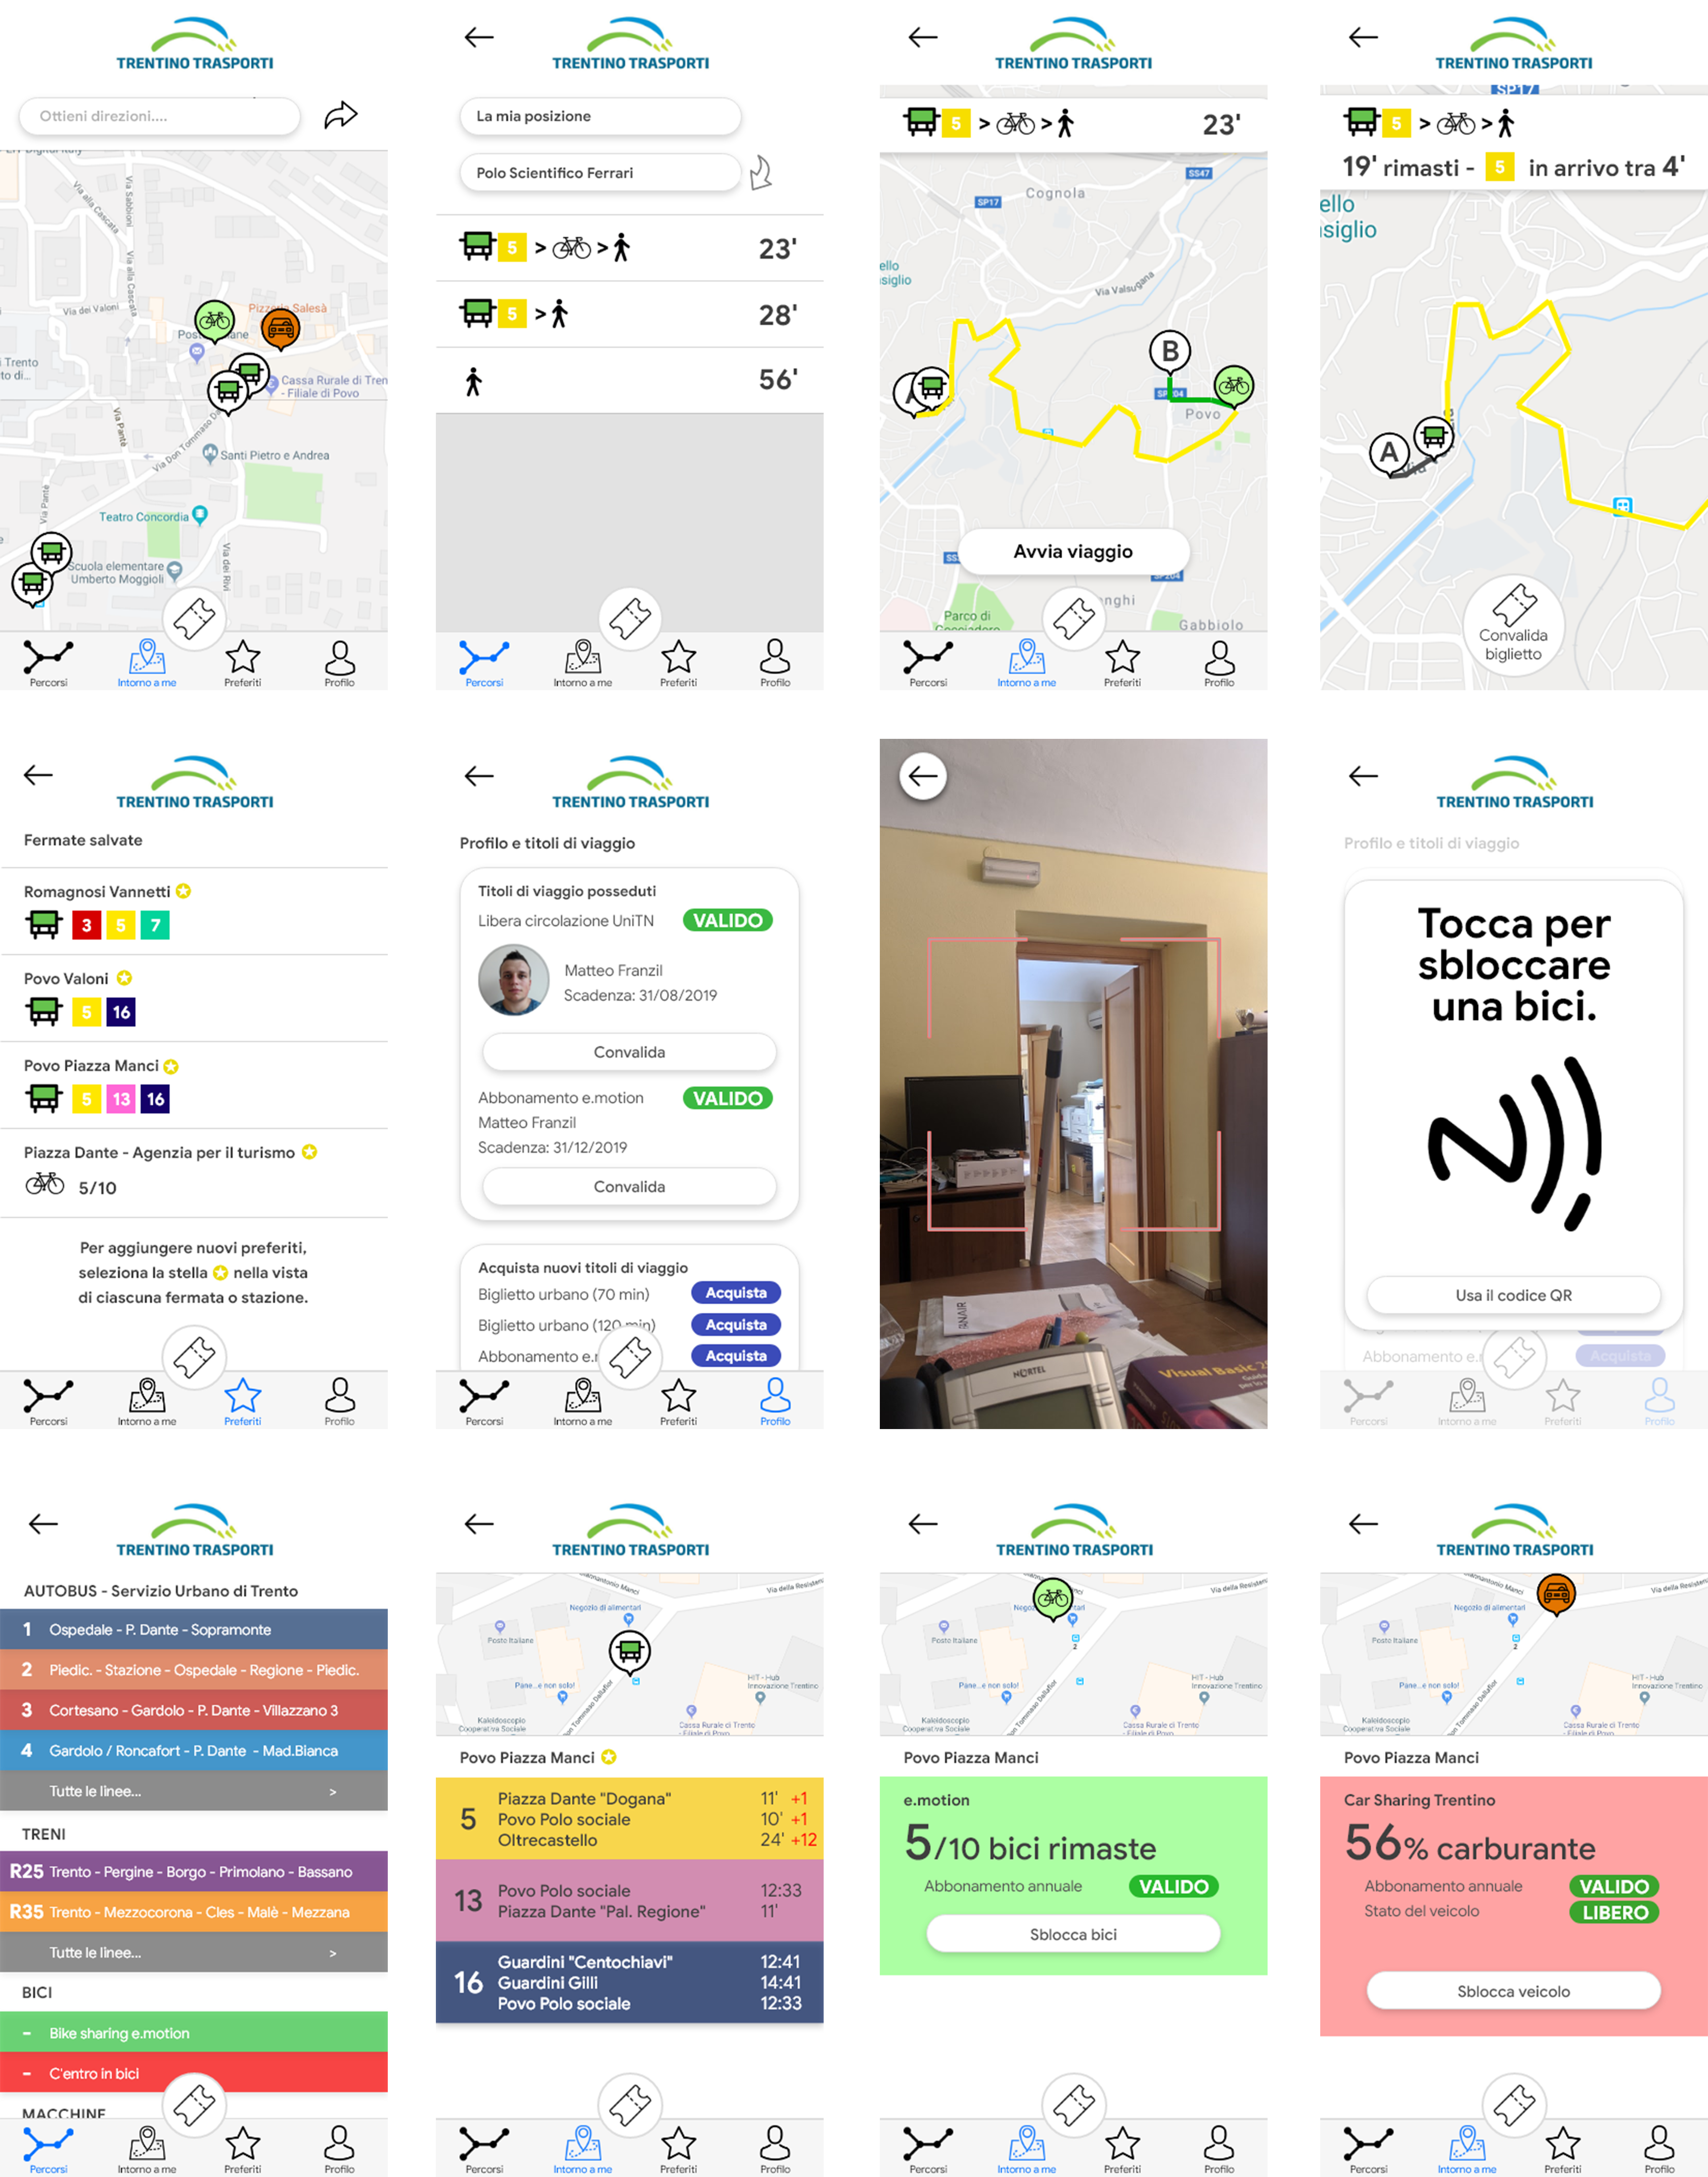
\includegraphics[width=\textwidth]{drawable/medfid/uniti}
    \caption{Medium fidelity prototype.}
    \label{fig:medfid}
\end{figure}

Figure \ref{fig:medfid}  shows the medium fidelity prototype. The interactive version can be found \href{https://xd.adobe.com/view/112eeb38-8c0f-4878-7d52-3e69ad2713bb-671f/?fullscreen}{by clicking here}, or at this url:\\\url{https://xd.adobe.com/view/112eeb38-8c0f-4878-7d52-3e69ad2713bb-671f/?fullscreen}.

As said above, most improvements in the second prototype focused on the Tickets and Directions view. A big, clear button was positioned at the center of the navigation bar, with the aim of validating as fast as possible any ticket in the user's possession.

The Directions view was completely reimagined, taking more inspiration from existing navigation apps such as \textit{Citymapper}. The focus is now more on the map, both in the initial view and in the turn-by-turn view, with clear indication of the remaining time and what the user has to do next.

I chose a white-dominant design, sticking to Google's \textit{Material Design 2} guidelines (that could be nonetheless be easily ported to other platforms). Transit options are coded with vibrant colors, especially in the map view; bus lines retain their color, assigned by \textit{Trentino trasporti}, in order to be quickly identified.

The Ticket menu was revamped, now showing options to buy additional tickets, but retaining priority to tickets already in possession.

\section{Evaluation of the medium fidelity prototype}

In order to conduct testing of the second prototype, I made use of Adobe XD's online feature in order to emulate the application on the users' smartphones, just as it was a regularly installed app.

People found the interface very intuitive and clear and welcomed the improvements to the Direction view. Some suggested the addition of real-time notifications to the app, which was clearly impossible in the prototype, but would be a nice improvement to the turn-by-turn experience.

Some people found \textit{Trentino trasporti}'s logo to be too invasive and should be reduced in size, something that I didn't think about during the design.

Other people, on the other hand, suggested the addition of a clearer way of inputting directions from point A from point B, since the current location is selected as default when looking for directions and the interface isn't completely clear on the purpose.

\section{Conclusion}

Firstly, in order for the project to succeed, this app needs to be heavily marketed, for example with flyers, billboards and bus advertisements, in order to cater to as much people as possible. At the same time, all the now redundant apps made by the Province, such as \textit{iBus}, \textit{ViaggiaTrento}, need to be taken out of the market, suggesting users to move to the newer alternative.

This may initially discourage some people, such as the elderly and the less experienced with smartphones; however, in the long run, if the app is deemed reliable, fast and intuitive, good word of mouth will spread and the app usage will increase accordingly, as long as the application is properly mantained.

Secondly, the app needs to be built in order to be as less resource intensive (therefore avoiding unneccessary features and cluttered) and to be supported by most smartphones on the market, for the same reasons stated above. This needs careful planning from a software development perspective.

Finally, it needs full support from all transit agencies involved, beginning from \textit{Trentino trasporti} and \textit{Trenitalia}. These companies need to provide data over a period of time (for example, real time information) and support for purchase of their tickets subscriptions. If this were not to happen, the whole project would need to be dropped from the very start.
\end{document}
